\documentclass[tikz,border=2pt]{standalone}
\usepackage{amsmath}
\usetikzlibrary{arrows.meta}
\begin{document}
% Global environment with x = 3 and functions f, g. The call f(4) has local y = 4, x = 5, z = 9 and
% returns 9 (global x unchanged); the call g(4) has no local x, looks up x = 3 outside and returns 7.
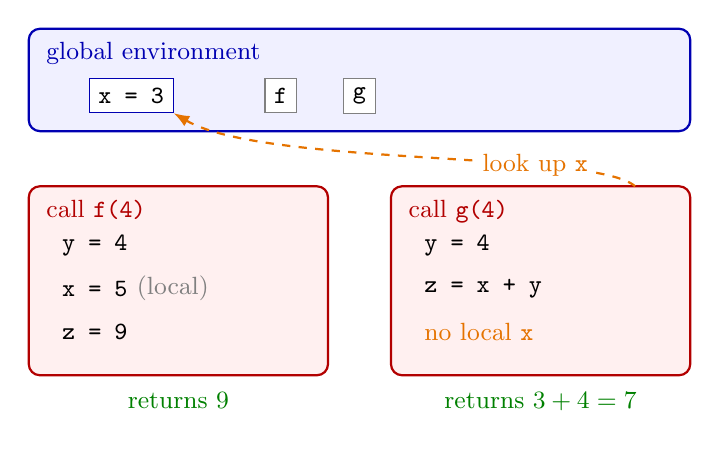
\begin{tikzpicture}[font=\small, >={Latex[length=2mm]},
  env/.style={draw, rounded corners=4pt, inner sep=5pt, align=left}]
  % global
  \draw[blue!70!black, thick, fill=blue!6, rounded corners=4pt] (0,0) rectangle (8.4,-1.3);
  \node[anchor=north west, blue!70!black] at (0.1,-0.05) {global environment};
  \node[draw=blue!70!black, fill=white, font=\small\ttfamily] (gx) at (1.3,-0.85) {x = 3};
  \node[draw=gray, fill=white, font=\small\ttfamily] at (3.2,-0.85) {f};
  \node[draw=gray, fill=white, font=\small\ttfamily] at (4.2,-0.85) {g};
  % call f(4)
  \draw[red!70!black, thick, fill=red!6, rounded corners=4pt] (0,-2.0) rectangle (3.8,-4.4);
  \node[anchor=north west, red!70!black] at (0.1,-2.05) {call \texttt{f(4)}};
  \node[anchor=west, font=\small\ttfamily] at (0.3,-2.75) {y = 4};
  \node[anchor=west, font=\small\ttfamily] (fx) at (0.3,-3.3) {x = 5};
  \node[anchor=west, gray] at (1.25,-3.3) {(local)};
  \node[anchor=west, font=\small\ttfamily] at (0.3,-3.85) {z = 9};
  % call g(4)
  \draw[red!70!black, thick, fill=red!6, rounded corners=4pt] (4.6,-2.0) rectangle (8.4,-4.4);
  \node[anchor=north west, red!70!black] at (4.7,-2.05) {call \texttt{g(4)}};
  \node[anchor=west, font=\small\ttfamily] at (4.9,-2.75) {y = 4};
  \node[anchor=west, font=\small\ttfamily] (gz) at (4.9,-3.3) {z = x + y};
  \node[anchor=west, orange!90!black] at (4.9,-3.85) {no local \texttt{x}};
  \draw[->, thick, dashed, orange!90!black] (7.7,-2.0) .. controls (7.2,-1.55) and (3.0,-1.75) .. (gx.south east)
     node[pos=0.3, fill=white, inner sep=1pt] {look up \texttt{x}};
  % returns
  \node[green!50!black, anchor=north] at (1.9,-4.5) {returns 9};
  \node[green!50!black, anchor=north] at (6.5,-4.5) {returns $3+4=7$};
\end{tikzpicture}
\end{document}
